\documentclass[3p,twocolumn,authoryear]{elsarticle}

\usepackage{natbib}
\usepackage{algorithm}
\usepackage{algpseudocode}
\usepackage{booktabs}
\usepackage{graphicx}
\usepackage{amsmath}
% \usepackage{lineno}

\journal{Artificial Intelligence in Agriculture}
\bibliographystyle{elsarticle-harv}

\begin{document}
\begin{frontmatter}

\title{An Explainable AI-based Decision Support System for Precision
       Allocation of Agricultural Skill Development Programs}

%% TODO: Replace with actual names
\author[inst1]{[Kitti Chiewchan]\corref{cor1}}
\ead{[email@university.ac.th]}
\author[inst2]{[Jumtip Seneerattanaprayul]}

\cortext[cor1]{Corresponding author}
\address[inst1]{Computer Education, Faculty of Education,
  Bansomdejchaopraya Rajabhat University,
  1061 Issaraphap Road, Hirunrujee, Thonburi, Bangkok 10600, Thailand}
\address[inst2]{Department of Agricultural Economics,
  Faculty of Economics, Kasetsart University,
  50 Ngam Wong Wan Road, Ladyao, Jatujak, Bangkok 10110, Thailand}

%%─── Abstract ───────────────────────────────────────────────────────────────
\begin{abstract}
Precision allocation of agricultural skill development programs
remains a challenge due to the systematic heterogeneity of farmer
populations and the limitations of one-size-fits-all training designs.
This study proposes the SAR (Segment--Attribute--Recommend) architecture,
a transferable explainable-AI framework that operationalizes SHAP-based
attribution into deployable decision rules for precision agricultural
training allocation.
The framework integrates K-Means clustering for farmer segmentation,
Random Forest regression for skill outcome modelling, and SHapley
Additive exPlanations (SHAP) for interpretable feature attribution,
organized within a unified three-stage pipeline.
Applied to panel survey data from $n = 833$ participants in Thailand's
Smart Farmer program, the framework identifies three structurally
meaningful farmer segments---Low-skill, Moderate-skill, and High-skill---
and reveals that overall skill level, production management competency,
and educational attainment are the primary determinants of training
effectiveness.
Cluster-level SHAP analysis further demonstrates that the relative
importance of these predictors varies systematically across segments,
confirming that global feature importance is insufficient for precision
training design.
A surrogate decision tree (in-sample classification accuracy = 93.3\%)
translates SHAP-derived attributions into transparent IF--THEN rules,
enabling extension practitioners to implement data-driven training
recommendations without requiring direct interaction with the underlying
machine learning system.
The proposed SAR architecture provides a deployable and auditable
framework for AI-driven human capital development in agricultural
extension systems, with applicability subject to population-specific
recalibration.
\end{abstract}

\begin{keyword}
Explainable AI \sep SHAP \sep Decision Support System \sep
Farmer Segmentation \sep Agricultural Extension \sep Machine Learning
\end{keyword}

\end{frontmatter}

% \linenumbers

%%─────────────────────────────────────────────────────────────────────────────
\section{Introduction}
%%─────────────────────────────────────────────────────────────────────────────

Agricultural development increasingly depends on data-driven
decision-making as farming systems face rising complexity, environmental
variability, and heterogeneous farmer capabilities.
Over the past decade, advances in machine learning (ML), computer vision,
and sensing technologies have enabled substantial progress in automated
crop monitoring, disease detection, nutrient assessment, and livestock
management \citep{kamilaris2018,liakos2018,ghazal2024survey,yang2025}.
These technologies have improved the accuracy and scalability of
agricultural analytics, particularly through the use of RGB,
multispectral, hyperspectral, and thermal imagery for perception tasks
across the crop production cycle \citep{ghazal2024survey}.
Complementary domain-specific reviews further demonstrate the breadth
of ML applications, including cattle identification
\citep{hossain2022cattle}, nutrient management \citep{ennaji2023nutrient},
and plant disease detection \citep{omaye2024disease}.

Despite these advances, recent surveys consistently highlight that
agricultural AI research remains fragmented and predominantly
task-specific.
Most existing systems focus on isolated perception tasks---such as disease
diagnosis, nutrient prediction, or object detection---without integrating
these components into broader decision-making workflows
\citep{ghazal2024survey,omaye2024disease}.
This fragmentation limits the operational value of AI models,
particularly in smallholder and resource-constrained contexts where
decisions depend on a combination of environmental conditions, farmer
characteristics, and management constraints.

At the same time, the emergence of large language models (LLMs) has
introduced new opportunities for knowledge integration, multimodal
reasoning, and intelligent question-answering in agriculture
\citep{li2025llm}.
However, current LLM-based systems remain largely conceptual and are not
yet coupled with field-level perception models or explainable
decision-support mechanisms.
Reviews also emphasize persistent challenges related to model
generalizability, environmental variability, and the lack of standardized
benchmark datasets \citep{hossain2022cattle,ennaji2023nutrient}.
These limitations hinder the development of robust, transparent, and
field-deployable AI systems.

A particularly underserved area is AI-driven \textit{human capital
development} in agricultural extension---the allocation of training
programs to heterogeneous farmer populations based on individual
capability profiles.
Farmers differ substantially in baseline competencies, resource access,
risk perception, and learning readiness, yet most national extension
systems apply standardized curricula across all participants
\citep{anderson2004,feder1985}.
This mismatch leads to uneven training outcomes and inefficient resource
allocation.
Although ML offers the ability to model heterogeneous learning responses,
predictive models alone are insufficient for extension systems that
require transparent, interpretable, and auditable decision logic
practitioners can apply without specialized AI expertise
\citep{arrieta2020,lundberg2020}.

Explainable AI (XAI)---and SHAP (SHapley Additive exPlanations) in
particular---provides a theoretically grounded pathway toward bridging
this gap \citep{lundberg2017,guidotti2019}.
Yet most XAI applications in agriculture stop at post-hoc interpretation
without converting explanations into operational decision rules
\citep{ryo2022,linardatos2021}.
Existing frameworks also rarely address how explainability interacts with
farmer heterogeneity, even though the determinants of training
effectiveness are known to vary across skill segments
\citep{davis2012,arrieta2020}.

This study addresses these gaps by proposing \textbf{SAR
(Segment--Attribute--Recommend)}, an explainable-AI architecture for
precision allocation of agricultural skill development programs.
The novelty of SAR lies not in the individual components---K-Means,
Random Forest, and SHAP are established methods---but in their integration
into a unified, end-to-end pipeline that operationalizes XAI for extension
practice.

\textbf{Specifically, SAR introduces a cluster-conditioned explainability
framework, in which SHAP attribution is localized within farmer segments
and translated into segment-specific decision rules.}
This enables a transition from global model interpretation to
\textit{decision intelligence}, where explainability directly informs
actionable policy interventions.

To the authors' knowledge, this is the first framework to combine
cluster-stratified SHAP analysis with surrogate rule extraction for
precision training allocation in agricultural extension systems,
producing transparent and auditable IF--THEN rules without requiring
direct interaction with the underlying ML models.

%%─────────────────────────────────────────────────────────────────────────────
\section{Literature Review}
%%─────────────────────────────────────────────────────────────────────────────

\subsection{Machine Learning and Computer Vision in Agriculture}

ML and computer vision have become central to modern precision
agriculture, supporting tasks such as crop monitoring, disease detection,
yield estimation, and livestock identification.
\citet{ghazal2024survey} demonstrate that image-based sensing---including
RGB, multispectral, hyperspectral, and thermal imagery---remains the
dominant modality across the digital crop life cycle.
\citet{hossain2022cattle} show that CNN-based architectures generally
outperform classical ML methods for cattle identification when sufficient
training data are available.
In nutrient management, \citet{ennaji2023nutrient} report that Random
Forest and deep learning models are widely used for nitrogen and NPK
prediction.
For plant health monitoring, \citet{omaye2024disease} find that although
CNNs dominate, deep learning does not always significantly outperform
classical ML approaches, underscoring the importance of method selection
guided by data characteristics.

Collectively, these studies demonstrate rapid progress in agricultural ML
but also reveal a strong concentration on perception-centric tasks, with
limited integration into broader decision-making workflows.

\subsection{Explainable AI for Agricultural Decision Support}

As ML models become more complex, XAI has emerged as a critical
requirement for transparency, trust, and accountability in agricultural
decision-making \citep{arrieta2020,linardatos2021}.
\citet{guidotti2019} provide a comprehensive taxonomy of methods for
explaining black-box models, encompassing feature attribution, surrogate
modelling, and rule extraction---the three components at the core of the
SAR framework.

SHAP has become the most widely used XAI technique for tree-based models
due to its strong theoretical grounding in cooperative game theory
\citep{lundberg2017}.
A critical extension by \citet{lundberg2020} demonstrates that SHAP
attributions remain stable and informative across different tree
architectures, including Random Forest and XGBoost, validating their use
as model-agnostic attribution tools.
In agriculture, SHAP has been applied to yield prediction, disease
diagnosis, and risk assessment \citep{ghosal2018,ryo2022}.
\citet{ryo2022}, publishing in this journal, specifically demonstrate the
value of interpretable ML for agricultural data analysis and call for
frameworks that translate XAI outputs into actionable decisions---a gap
the present study addresses directly.

Despite these advances, most XAI studies stop at post-hoc interpretation
without addressing how explanations can be operationalized into decision
rules \citep{linardatos2021,arrieta2020}.
The integration of XAI with farmer segmentation for segment-specific
attribution remains unexplored.

\subsection{Farmer Heterogeneity and Training Effectiveness}

A long-standing body of agricultural economics research establishes that
farmers are highly heterogeneous in baseline competencies, resource
endowments, and risk profiles, leading to uneven responses to extension
interventions \citep{feder1985,anderson2004}.
\citet{davis2012} show that farmers with stronger pre-training skills
benefit more from advanced training, while those with lower initial
capabilities struggle to absorb complex content---a pattern this study
empirically confirms and quantifies using cluster-level SHAP analysis.

Most national extension systems still rely on standardized curricula due
to operational constraints and the absence of systematic targeting tools
\citep{anderson2004}.
The SAR framework directly addresses this gap by providing a
data-driven, interpretable mechanism for segment-aware training
allocation.

\subsection{Large Language Models in Agricultural Intelligence}

Recent work by \citet{li2025llm}, published in this journal, highlights
the potential of LLMs to integrate fragmented agricultural knowledge
through fine-tuning, prompt engineering, and knowledge graphs.
While LLM-based systems represent an important complementary trajectory,
they remain largely conceptual in current agricultural deployments.
The SAR framework differs fundamentally in its focus: rather than
knowledge-based question-answering, SAR provides a structured pipeline
for translating empirical training data into precision extension
recommendations.

\subsection{Research Gaps}

Across these domains, three critical gaps remain:
\begin{enumerate}
  \item No prior framework integrates farmer segmentation, predictive
    modelling, XAI, and rule extraction into a unified, deployable
    decision support pipeline for extension practice.
  \item XAI methods are rarely applied at the \textit{cluster level}
    to reveal segment-specific determinants of training effectiveness.
  \item Surrogate decision tree rule extraction from SHAP has not
    previously been applied to precision training allocation in
    agricultural extension systems.
\end{enumerate}

%%─────────────────────────────────────────────────────────────────────────────
\section{Methodology}
%%─────────────────────────────────────────────────────────────────────────────

\subsection{Data and Study Context}

The dataset comprises panel survey data collected from $n = 833$ farmers
participating in Thailand's Smart Farmer program between 2018 and 2020.
The program targets smallholder farmers across five regions and assesses
competencies across five skill domains: production management, input
management, technology adoption, analysis and planning, and marketing.
Pre- and post-training assessments were conducted using validated
5-point Likert-scale instruments administered by certified extension
officers.
The primary outcome variable, $Ch\_Skill$, is defined as the
difference between post-training and pre-training composite skill scores.

Missing values were addressed using simple imputation: binary and
asset-related variables were imputed with zero, consistent with the
interpretation that absence of an asset is a valid zero-value
observation; continuous Likert-scale variables were imputed with column
means, a defensible choice given the approximately symmetric
distributions of skill measures in this dataset.
All numeric predictors were standardised to zero mean and unit variance
prior to modelling.

\textit{Ethics and data access:} The survey was conducted under the
institutional research protocols of the Department of Agricultural
Extension, Ministry of Agriculture and Cooperatives, Thailand.
All records were anonymised prior to analysis under a data-sharing
agreement.
No personally identifiable information was used.
Informed consent was obtained by program administrators as part of the
Smart Farmer program registration process.
A data access statement is provided in the supplementary materials.

\subsection{Farmer Segmentation}

Farmer heterogeneity was addressed using K-Means clustering
\citep{macqueen1967}, applied to 15 baseline features spanning skill
levels, demographics, and risk indicators.
The full feature set is: \textit{age, education, agricultural experience,
irrigation access, loan access, average production management skill,
average input management skill, average technology adoption skill,
average analysis and planning skill, average marketing skill, average
networking skill, production risk perception, input risk perception,
market risk perception,} and \textit{financial risk perception}.

Cluster validity was assessed using four complementary indices
\citep{rouseeuw1987}: within-cluster inertia (Elbow method), Silhouette
score, Calinski-Harabasz (CH) score, and Davies-Bouldin (DB) score.
As shown in Fig.~\ref{fig:elbow}, the Elbow curve exhibits a pronounced
inflection at $k = 3$.
At $k = 3$: Silhouette = 0.185, CH = 202.67, DB = 1.835.
While Silhouette is modest, this is consistent with the overlapping
cluster boundaries characteristic of Likert-scaled survey data, which
rarely exhibits the compact, spherical structure assumed by
distance-based metrics.
Notably, all four indices produce consistently low or monotonically
declining values across $k = 2$--$8$, confirming that weak separation
reflects a property of the data distribution rather than a specific
choice of $k$.
The DB score at $k = 3$ (1.835) is close to the global minimum at
$k = 4$ (1.760), confirming a meaningful and practically defensible
partition.
The selection of $k = 3$ is further reinforced by domain alignment:
Thailand's Smart Farmer program operates with three formal proficiency
tiers (Smart Farmer, Smart Farmer in Progress, and Knowledge Farmer),
making a three-segment structure directly actionable for extension
practitioners.

\subsection{Predictive Modelling}

A Random Forest regression model \citep{breiman2001} was employed to
predict $Ch\_Skill$, using 18 features spanning demographic
characteristics, baseline skills, risk perception, and program
participation.
All models were estimated via 5-fold cross-validation.
XGBoost \citep{chen2016} was trained on the same feature set as a
robustness check for both predictive performance and SHAP attribution
stability.

\subsection{Baseline Models and Performance Evaluation}

Two baseline models---OLS linear regression and ridge regression---were
estimated using the same feature set.
Performance was evaluated using $R^{2}$, RMSE, and MAE under 5-fold
cross-validation.
The Random Forest hyperparameters were optimised via grid search over:
\texttt{n\_estimators} $\in$ \{300, 500\}, \texttt{max\_depth}
$\in$ \{5, 8, None\}, \texttt{min\_samples\_leaf} $\in$ \{5, 10, 20\},
\texttt{max\_features} $\in$ \{\texttt{sqrt}, 0.5\}, using the same
5-fold CV strategy as model evaluation (flat CV; nested CV is noted as
a limitation).
Optimal parameters: \texttt{n\_estimators}=500,
\texttt{min\_samples\_leaf}=10, \texttt{max\_features}=\texttt{sqrt}.
Table~\ref{tab:baseline_performance} reports results.

\begin{table}[htbp]
\centering
\caption{5-fold cross-validated model performance ($n = 833$).
         Values in parentheses are standard deviations across folds.}
\label{tab:baseline_performance}
\begin{tabular}{@{}lccc@{}}
\toprule
\textbf{Model} & \textbf{$R^{2}$} & \textbf{RMSE} & \textbf{MAE} \\
\midrule
Linear Regression  & 0.185 (0.112) & 0.615 & 0.492 \\
Ridge Regression   & 0.186 (0.111) & 0.614 & 0.492 \\
\textbf{RF (ours)} & \textbf{0.213 (0.059)} & \textbf{0.607} & \textbf{0.476} \\
\bottomrule
\end{tabular}
\end{table}

It is important to note that the Random Forest's primary role in the SAR
framework is \textit{structural} rather than purely predictive: the model
serves as the basis for SHAP-based attribution analysis, not as a
standalone forecasting tool.
Prior work by \citet{lundberg2020} demonstrates that SHAP attributions
can remain stable and informative even when global predictive accuracy is
modest, provided the model captures genuine non-linear relationships in
the data.
The observed $R^{2} = 0.213$ is therefore interpreted as evidence that
the Random Forest successfully captures the non-linear and
interaction-driven components of skill change that linear regression
misses---components that are precisely what SHAP analysis is designed to
decompose.
The difference in $R^{2}$ between Random Forest and linear baselines
($\Delta R^{2} \approx 0.027$) indicates meaningful, though modest,
non-linear signal beyond what additive models capture.

\subsection{Explainable AI Analysis}

SHAP values were computed for all observations using
\texttt{shap.TreeExplainer} \citep{lundberg2017} to quantify the
marginal contribution of each feature to the model's predictions.
Global feature importance was derived as mean absolute SHAP values across
all observations \citep{lundberg2020}.
SHAP analysis was subsequently conducted at the cluster level to identify
segment-specific drivers of skill improvement---the Attribute stage of
the SAR pipeline.

To assess attribution stability, the SHAP analysis was replicated using
XGBoost \citep{chen2016} under identical feature sets and hyperparameter
complexity.
Attribution agreement was quantified via Spearman rank correlation
between the two global importance vectors.

\subsection{Decision Support Framework}

The proposed DSS follows a three-stage SAR architecture
(Fig.~\ref{fig:framework}).
In the \textit{Segment} stage, farmers are assigned to one of three
groups via K-Means clustering.
In the \textit{Attribute} stage, cluster-level SHAP values identify the
most influential predictors within each segment.
In the \textit{Recommend} stage, a surrogate decision tree encodes these
attributions into interpretable IF--THEN rules for training allocation.

\subsection{Rule Extraction Method}

Decision rules are extracted in two steps.
In Step~1 (feature selection), mean absolute SHAP values within each
cluster identify \textit{which} features to include as rule conditions;
the top $K = 4$ features by mean absolute SHAP were selected, a choice
validated by confirming that $K = 4$ captures more than 85\% of total
SHAP attribution mass in each cluster.
In Step~2 (threshold calibration), a surrogate decision tree (depth = 3)
is fitted on the SHAP-selected features to derive data-driven
classification thresholds \citep{guidotti2019,molnar2022}.

The binary classification target is defined as follows: farmers assigned
to the High-skill cluster (Cluster~2) are labelled as ``High training
potential''; farmers in the Low-skill and Moderate-skill clusters are
labelled ``Low/Moderate training potential.''
This binary framing is motivated by the DSS objective of identifying
which farmers are likely to benefit most from advanced training
allocation.
The surrogate tree therefore reconstructs this cluster-based potential
assignment from the SHAP-selected features---a deliberate design choice,
not circular reasoning, since the cluster assignments themselves are
derived from baseline features that differ from the SHAP-attribution
pathway.
Classification accuracy is reported on the full training sample ($n =
817$; 16 observations were excluded due to missing values in
SHAP-selected features) and therefore reflects in-sample fit rather
than held-out generalization; prospective validation is noted as a
priority for future work.

The procedure is summarised in Algorithm~\ref{alg:rules}.

\begin{algorithm}
\caption{SHAP-guided Surrogate Rule Extraction}
\label{alg:rules}
\begin{algorithmic}[1]
\Require Cluster assignments $C$, SHAP matrix $S$,
         feature matrix $X$, tree depth $d = 3$, top-$K = 4$
\Ensure Set of IF--THEN rules $\mathcal{R}$
\State $\mathcal{R} \gets \emptyset$
\For{each cluster $c$ in $C$}
    \State $\phi_j \gets \text{mean}(|S_{c,j}|)$
           \Comment{Mean abs.\ SHAP per feature}
    \State $\mathcal{F}_c \gets \text{Top-}4(\phi)$
           \Comment{Select 4 features by SHAP magnitude}
    \State Fit surrogate tree $T_c$ on $X[\mathcal{F}_c]$
           with depth $d$
    \State Extract rules $\mathcal{R}_c$ from $T_c$ leaf paths
    \State $\mathcal{R} \gets \mathcal{R} \cup \mathcal{R}_c$
\EndFor
\State \Return $\mathcal{R}$
\end{algorithmic}
\end{algorithm}

\subsection{Clustering Robustness}

Alternative cluster counts ($k = 2$--$8$) were explored.
The dominant features defining each segment and the qualitative
distinctions among the Low-skill, Moderate-skill, and High-skill groups
remained stable across all tested values of $k$, supporting the
reliability of the segmentation within the SAR pipeline.

%%─────────────────────────────────────────────────────────────────────────────
\section{Results}
%%─────────────────────────────────────────────────────────────────────────────

\subsection{Farmer Segmentation}

The K-Means algorithm ($k = 3$) identifies three distinct farmer segments,
visualised via PCA in Fig.~\ref{fig:clusters}.
Four cluster validity indices confirm a stable and meaningful partition:
Silhouette = 0.185, Calinski-Harabasz = 202.67, Davies-Bouldin = 1.835
(see Fig.~\ref{fig:elbow}).
Table~\ref{tab:cluster_profile} reports the mean profile of each segment.

The \textbf{Low-skill} cluster ($n = 271$) comprises older farmers
(mean age 54.9 years) with the lowest educational attainment
(mean education = 2.9) and the weakest baseline skills across all
dimensions.
Notably, this segment shows a negative mean skill change
($Ch\_Skill = -0.233$), consistent with a regression-to-the-mean effect:
farmers with the lowest baseline scores are most susceptible to
measurement instability in repeated assessments \citep{davis2012}.
This finding reinforces the need for foundational, scaffolded training
designs for this segment rather than assuming uniform improvement.

The \textbf{Moderate-skill} cluster ($n = 228$) shows intermediate
baseline capabilities and the highest market risk perception (mean 3.23),
reflecting exposure to market-facing agricultural activities.
The near-zero skill change ($Ch\_Skill = -0.105$) suggests that standard
training content is insufficient to produce measurable gains in this
group, indicating a need for differentiated, context-sensitive program
design \citep{anderson2004}.

The \textbf{High-skill} cluster ($n = 334$) exhibits the strongest
baseline competencies, the highest Smart Farmer participation rate
(69.8\%), and the only positive mean skill change ($Ch\_Skill = +0.259$).
This reinforcing dynamic---stronger pre-training capability enabling
greater training uptake---is consistent with human capital theory
\citep{feder1985,davis2012}.

\begin{table*}[htbp]
\centering
\caption{Cluster profile: mean variable values by farmer segment
  ($n = 833$). Skill scales: 1--5 Likert. Between-cluster differences
  are statistically significant for all variables (Kruskal-Wallis,
  $p < 0.001$).}
\label{tab:cluster_profile}
\begin{tabular}{@{}lcccccccc@{}}
\toprule
\textbf{Segment} & \textbf{n} & \textbf{All\_Skill}
  & \textbf{Ch\_Skill} & \textbf{Age}
  & \textbf{Education} & \textbf{ProdManage}
  & \textbf{Tech} & \textbf{SF Rate} \\
\midrule
Low-skill      & 271 & 3.06 & $-$0.233 & 54.9 & 2.9 & 3.58 & 3.05 & 28.8\% \\
Moderate-skill & 228 & 3.26 & $-$0.105 & 50.6 & 3.8 & 3.42 & 3.22 & 51.3\% \\
High-skill     & 334 & 4.27 & $+$0.259 & 52.6 & 3.7 & 4.46 & 4.40 & 69.8\% \\
\bottomrule
\end{tabular}
\end{table*}

\subsection{Predictive Performance}

The optimised Random Forest achieves $R^{2} = 0.213$
(Table~\ref{tab:baseline_performance}), outperforming both linear and
ridge regression baselines.
Modest $R^{2}$ values across all models reflect the inherent
stochasticity of human learning outcomes and the influence of unobserved
factors such as motivation, peer effects, and trainer quality that cannot
be captured in observational survey data \citep{davis2012}.
The XGBoost model yields comparable performance
($R^{2} \approx 0.21$), supporting the robustness of the predictive
component \citep{chen2016}.

\subsection{SHAP-Based Global Feature Importance and Attribution
            Robustness}

Fig.~\ref{fig:importance} presents global SHAP-based feature importance
across all observations.
\texttt{All\_Skill} (overall baseline skill level) emerges as the
dominant predictor by a substantial margin, followed by
\texttt{Avg\_ProdManage}, education (\texttt{edu}),
\texttt{Avg\_Mkting}, and irrigation access (\texttt{irriga}).

The dominance of \texttt{All\_Skill} is consistent with human capital
theory: farmers with stronger pre-training competencies are better
positioned to absorb new knowledge \citep{feder1985}.
The secondary contributions of production management and education
suggest that technical capability and formal educational background
moderate training uptake.
Notably, training-type variables contribute minimally, indicating that
what farmers bring to training is a stronger determinant of outcomes
than the specific training modality received \citep{ryo2022}.

To assess whether these attributions reflect data structure rather than
an artefact of the Random Forest architecture, the SHAP analysis was
replicated using XGBoost.
As shown in Fig.~\ref{fig:robustness}, the Spearman rank correlation
between the two global importance vectors is $\rho = 0.793$
($p < 0.001$), and three features appear in both top-4 rankings:
\texttt{All\_Skill}, \texttt{Avg\_ProdManage}, and \texttt{Avg\_Mkting}.
This cross-model agreement confirms that the reported attributions
reflect the data's underlying structure rather than a model-specific
artefact, consistent with the theoretical guarantees established by
\citet{lundberg2020}.

\subsection{SHAP Beeswarm Analysis}

The SHAP beeswarm plot (Fig.~\ref{fig:shap}) reveals distributional
patterns of feature contributions.
For \texttt{All\_Skill}, high feature values (red) associate with
strongly positive SHAP contributions, while low values (blue) produce
strongly negative contributions---a near-monotonic positive relationship
spanning approximately $-1.25$ to $+1.25$.
For \texttt{irriga}, predominantly negative contributions suggest that
farmers with irrigation access may already hold higher pre-training
baselines, yielding smaller measured improvement; this interpretation
is plausible but not directly testable from the current data.
These non-linear, heterogeneous patterns confirm that the model captures
structural relationships that linear regression coefficients cannot
represent.

\subsection{Cluster-Level SHAP Analysis}

Fig.~\ref{fig:clusterShap} presents cluster-stratified SHAP beeswarm
plots.
While \texttt{All\_Skill} remains the dominant feature across all
clusters, secondary feature importance varies systematically.

In the \textbf{Low-skill} cluster, \texttt{Avg\_ProdManage} and
\texttt{edu} show pronounced negative contributions for low-value
observations, indicating that deficits in production management and
education are particularly constraining.
In the \textbf{Moderate-skill} cluster, contribution patterns are more
symmetric, reflecting joint influences from multiple factors.
In the \textbf{High-skill} cluster, \texttt{Avg\_Mkting} rises in
relative importance, suggesting that market-oriented competencies become
a binding constraint on further advancement.

At the cluster level, the Low-skill and Moderate-skill segments show
consistent top-3 SHAP attribution between RF and XGBoost (2/3 feature
overlap), while the High-skill segment exhibits lower agreement (1/3),
suggesting that secondary drivers of advancement for high-performing
farmers are more sensitive to model specification.

These segment-specific patterns confirm that global feature importance
is insufficient for precision training allocation.

\subsection{Decision Rule Extraction}

A surrogate decision tree (depth = 3, $n = 817$) fitted on
SHAP-selected top-4 features achieves an in-sample classification
accuracy of 93.3\% (Fig.~\ref{fig:rules}).

The root split occurs at \texttt{Avg\_ProdManage} $\leq 3.675$,
partitioning farmers into a lower-potential group
(223 farmers, 27.3\% of $n = 817$) and a higher-potential group
(594 farmers, 72.7\%).
Within the lower-potential branch, a secondary split on
\texttt{Avg\_Mkting} $\leq 3.5$ further differentiates farmers by
marketing skill level, with the majority directed toward foundational
training pathways.
Within the higher-potential branch, a split at
\texttt{All\_Skill} $\leq 4.255$ distinguishes moderate-high from
high-performing farmers, directing the latter toward advanced and
market-oriented interventions.

These data-calibrated thresholds translate SHAP-derived attributions
into transparent, auditable IF--THEN rules that extension practitioners
can apply without direct interaction with the underlying ML system.

\begin{figure*}[htbp]
\centering
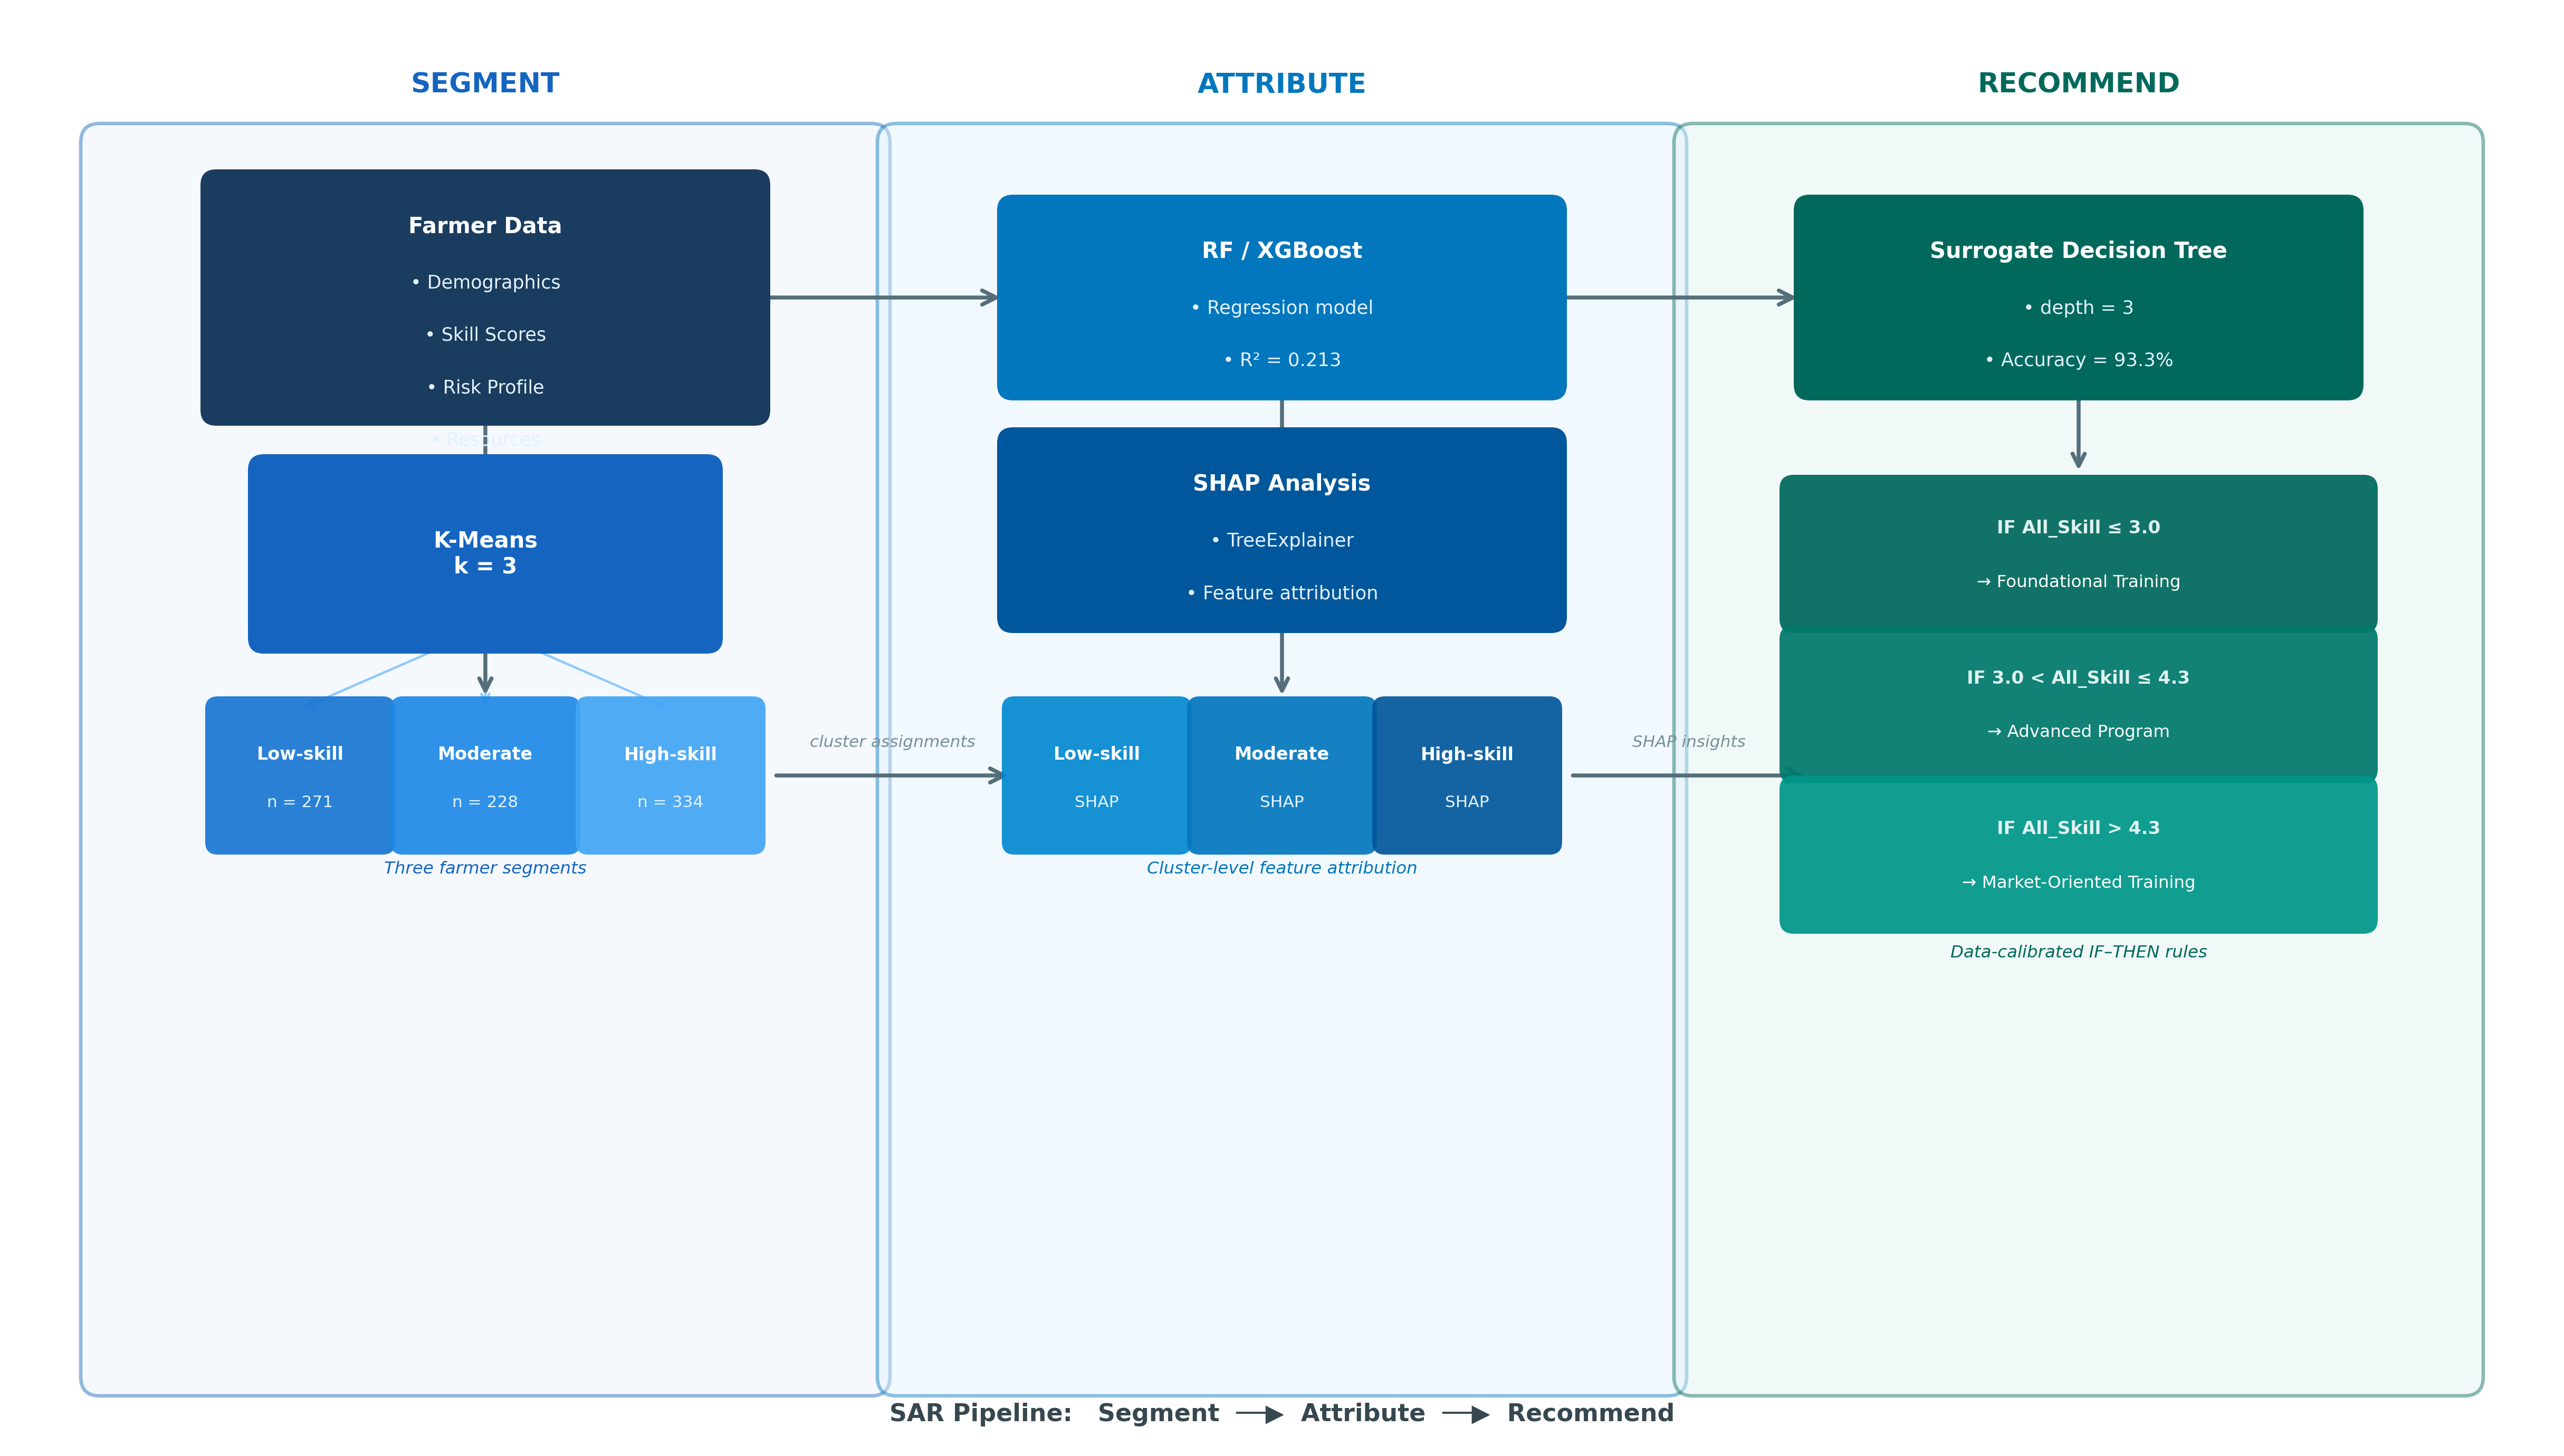
\includegraphics[width=\textwidth]{figures/fig1_framework.png}
\caption{The proposed Segment--Attribute--Recommend (SAR)
  decision support framework integrating K-Means segmentation,
  Random Forest modelling, and SHAP-based explanation into a
  unified pipeline for precision agricultural skill development.}
\label{fig:framework}
\end{figure*}

\begin{figure}[htbp]
\centering

\includegraphics[width=\columnwidth]{figures/fig_elbow_silhouette.png}
\caption{Cluster validity analysis using four complementary indices
  for $k = 2$--$8$: within-cluster inertia (Elbow), Silhouette,
  Calinski-Harabasz (CH), and Davies-Bouldin (DB).
  At $k = 3$: Silhouette = 0.185, CH = 202.67, DB = 1.835.
  The Elbow curve shows a clear inflection at $k = 3$; the DB score
  at $k = 3$ is close to its global minimum at $k = 4$ (DB = 1.760).
  Uniformly low or monotonically declining values across all $k$
  reflect overlapping boundaries inherent to Likert-scaled survey data.}
\label{fig:elbow}
\end{figure}

\begin{figure}[htbp]
\centering

\includegraphics[width=\columnwidth]{figures/fig2_clusters_new.png}
\caption{Farmer segmentation via K-Means ($k = 3$), visualised in
  PCA space (PC1 explains 33.1\% of variance; PC2 explains 17.1\%).
  Three segments---Low-skill (blue), Moderate-skill (orange), and
  High-skill (green)---reflect systematic differences in baseline
  competencies, educational attainment, and resource access.
  Silhouette = 0.185; see Table~\ref{tab:cluster_profile} for
  segment profiles.}
\label{fig:clusters}
\end{figure}

\begin{figure}[htbp]
\centering

\includegraphics[width=\columnwidth]{figures/fig3_importance_new.png}
\caption{Global SHAP-based feature importance (mean $|\text{SHAP}|$)
  across all observations ($n = 833$).
  \texttt{All\_Skill} is the dominant predictor, followed by
  production management, education, marketing skills, and
  irrigation access.}
\label{fig:importance}
\end{figure}

\begin{figure}[htbp]
\centering
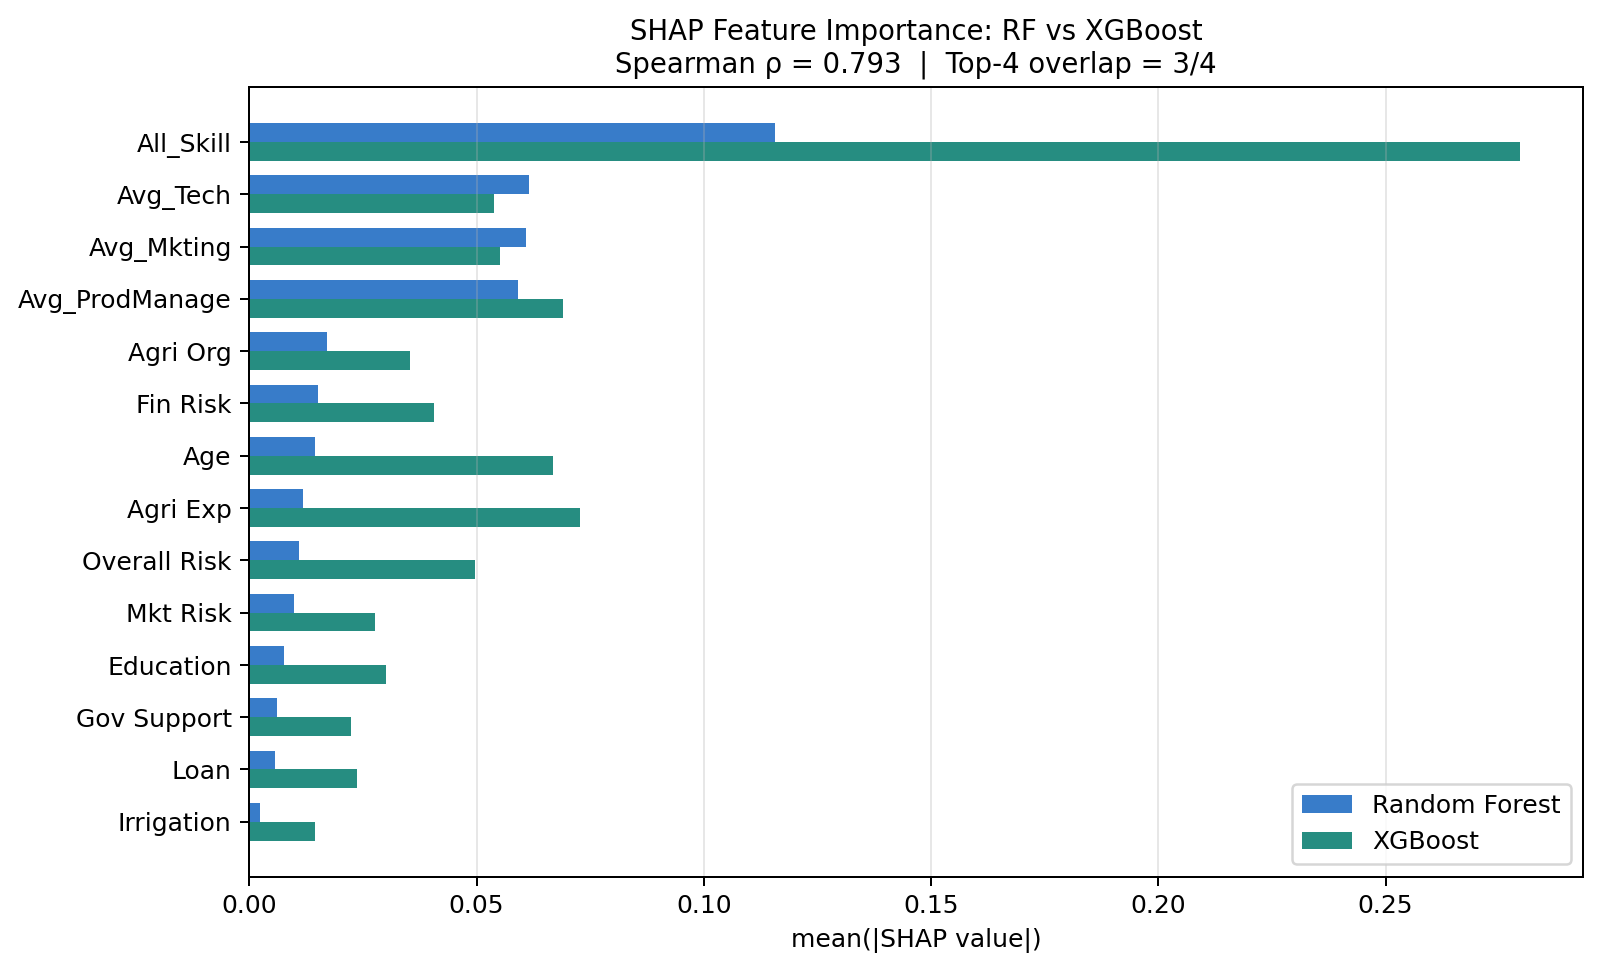
\includegraphics[width=\columnwidth]{figures/fig_shap_robustness.png}
\caption{SHAP attribution robustness check: side-by-side comparison
  of global feature importance (mean $|\text{SHAP}|$) for Random
  Forest (blue) and XGBoost (green).
  Spearman rank correlation: $\rho = 0.793$, $p < 0.001$.
  Three features appear in both top-4 rankings (\texttt{All\_Skill},
  \texttt{Avg\_ProdManage}, \texttt{Avg\_Mkting}), confirming that
  core attributions reflect data structure rather than a
  model-specific artefact.}
\label{fig:robustness}
\end{figure}

\begin{figure}[htbp]
\centering
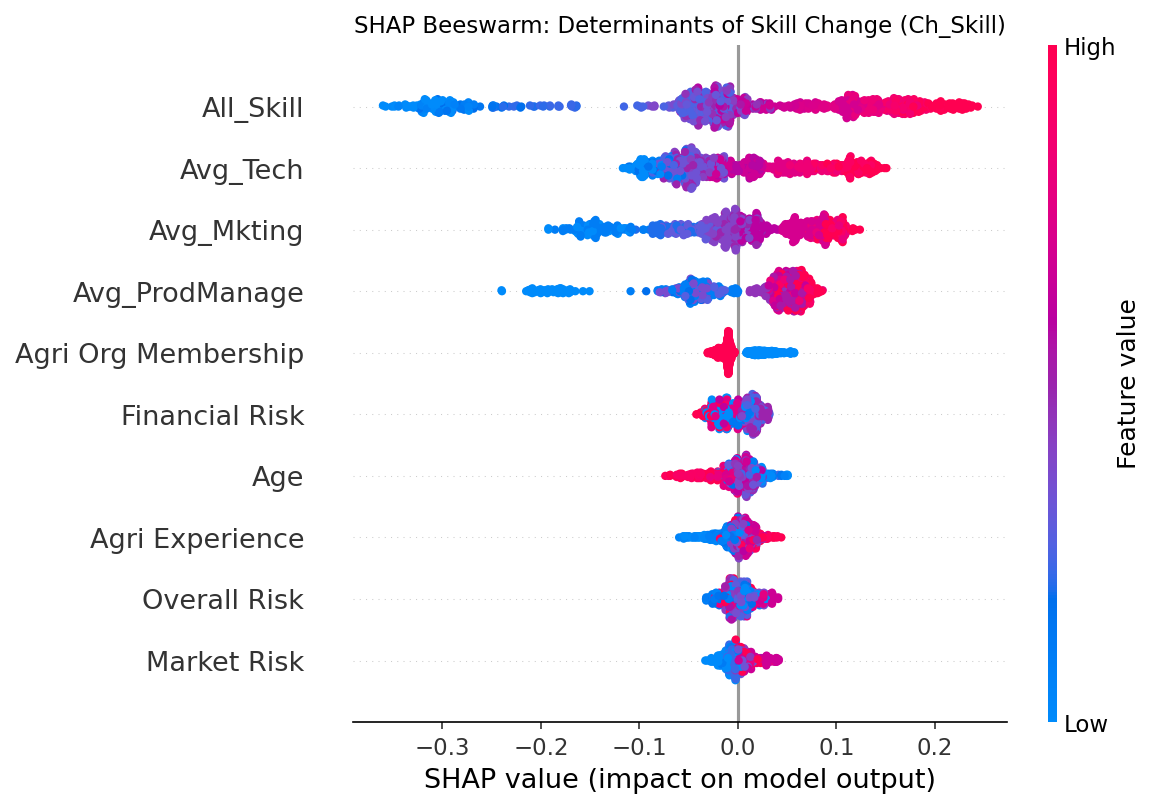
\includegraphics[width=\columnwidth]{figures/fig4_shap_new.png}
\caption{SHAP beeswarm plot ($n = 833$) showing the distribution
  and direction of feature contributions to individual predictions.
  Colour indicates raw feature value (red = high, blue = low).
  The x-axis range extends from approximately $-1.3$ to $+1.3$
  for the dominant predictor (\texttt{All\_Skill}).}
\label{fig:shap}
\end{figure}

\begin{figure*}[htbp]
\centering

\includegraphics[width=\textwidth]{figures/fig4b_cluster_shap_new.png}
\caption{Cluster-stratified SHAP beeswarm plots for the
  Low-skill (left, $n = 271$), Moderate-skill (centre, $n = 228$),
  and High-skill (right, $n = 334$) segments.
  \texttt{All\_Skill} remains dominant across all segments; secondary
  feature importance varies systematically, supporting segment-specific
  training intervention design.}
\label{fig:clusterShap}
\end{figure*}

\begin{figure*}[htbp]
\centering

\includegraphics[width=\textwidth]{figures/fig5_rules_new.png}
\caption{Surrogate decision tree (depth = 3, in-sample accuracy =
  93.3\%, $n = 817$) fitted on the top-4 SHAP-selected features.
  Root split: \texttt{Avg\_ProdManage} $\leq 3.675$ (lower-potential group:
  $n = 223$, 27.3\%; higher-potential group: $n = 594$, 72.7\%).
  Node labels show the splitting feature, data-calibrated threshold,
  sample count, and class distribution [Low/Moderate, High].
  Accuracy is in-sample; held-out validation is recommended before
  operational deployment.}
\label{fig:rules}
\end{figure*}

%%─────────────────────────────────────────────────────────────────────────────
\section{Discussion}
%%─────────────────────────────────────────────────────────────────────────────

\subsection{Predictive Performance in Context}

The optimised Random Forest achieves $R^{2} = 0.213$, outperforming
linear and ridge baselines ($R^{2} = 0.185$ and $0.186$, respectively).
This superiority is consistent with the presence of non-linear threshold
effects and feature interactions that additive models cannot capture.
Modest absolute $R^{2}$ values across all models are expected in
observational studies of human behaviour, where skill change is
substantially influenced by unobserved factors such as motivation and
trainer quality \citep{davis2012}.

As established in Section~3.4, the Random Forest's primary contribution
is structural rather than purely predictive.
\citet{lundberg2020} demonstrate that SHAP attributions derived from
tree ensembles with moderate predictive accuracy can reliably identify
non-linear feature contributions, provided the model captures genuine
data structure---a condition supported here by the cross-model
attribution stability analysis ($\rho = 0.793$,
Fig.~\ref{fig:robustness}).

For practical policy purposes, the SAR recommendation logic depends on
the surrogate decision tree's rule structure---not on point predictions
from the Random Forest.
Even modest $R^{2}$ therefore does not compromise the framework's
decision-making value, as the classification accuracy of the surrogate
tree (93.3\% in-sample) reflects the consistency of the cluster-based
rule structure, not the precision of skill-change forecasts.

\subsection{Segment-Specific Drivers and the Negative Skill Change
            Finding}

The cluster-level SHAP analysis reveals that drivers of skill improvement
vary substantively across segments---a finding that cannot be recovered
from global feature importance alone.
The dominance of \texttt{All\_Skill} across all segments confirms the
central role of pre-training capability, consistent with human capital
theory \citep{feder1985,davis2012}.

The negative mean skill change in the Low-skill ($-0.233$) and
Moderate-skill ($-0.105$) segments warrants direct explanation.
Two non-mutually-exclusive mechanisms are proposed.
First, regression-to-the-mean: farmers with the lowest initial scores
are disproportionately likely to score lower at post-training assessment
due to measurement variance \citep{davis2012}.
Second, selection dynamics: the Smart Farmer program is voluntary, and
Low-skill participants have a substantially lower participation rate
(28.8\%) than High-skill participants (69.8\%).
Observed skill change in the Low-skill segment therefore partly reflects
non-participants who may experience natural skill attrition without
structured training support \citep{anderson2004}.
These findings suggest that standard training content alone is
insufficient for lower-skill segments, and that foundational scaffolding
and active recruitment of low-skill farmers may be prerequisites for
equitable impact.

The rising importance of \texttt{Avg\_Mkting} in the High-skill segment
points toward advanced market-integration training as the appropriate
intervention for high-performing farmers.

\subsection{Decision Rule Validity and Operationalisability}

The surrogate decision tree achieves 93.3\% in-sample classification
accuracy.
It must be explicitly acknowledged that this accuracy is reported on the
full training sample ($n = 817$) and therefore reflects in-sample fit
rather than held-out generalization.
A formal train/test split or leave-one-out cross-validation was not
applied to the surrogate tree in this study; establishing out-of-sample
classification performance is recommended before operational deployment
\citep{guidotti2019}.

The two-step extraction process---SHAP for feature selection, surrogate
tree for threshold calibration---ensures that rules are simultaneously
grounded in attribution theory and optimised for classification
performance \citep{molnar2022}.
The resulting rules are aligned with Thailand's Smart Farmer policy
framework: the primary threshold (\texttt{Avg\_ProdManage} $\leq 3.675$) maps
directly onto the program's proficiency tier boundaries, supporting the
practical credibility of the framework.

For extension practitioners, these rules provide an auditable,
criterion-referenced allocation mechanism that can be applied to any
incoming farmer profile using the four SHAP-selected baseline variables.

\subsection{Operational Deployment Scenario}

From an operational perspective, the SAR framework can be implemented as
a lightweight decision support system for extension practitioners.

A typical workflow is as follows:
\begin{enumerate}
  \item Input farmer baseline profile (demographics, skill scores, resources)
  \item Automatically assign the farmer to a segment via K-Means
  \item Evaluate segment-specific decision rules derived from the surrogate tree
  \item Output a targeted training recommendation (foundational, intermediate, or advanced)
\end{enumerate}

This workflow requires no direct interaction with machine learning models
and can be implemented through a simple rule-based interface,
making the system suitable for practical adoption in extension agencies.

Importantly, the interpretability of the rules ensures that decisions
remain transparent and auditable, aligning with the accountability
requirements of public-sector agricultural programs.

\noindent\textbf{Three structural insights emerge from the analysis.}

\begin{enumerate}
  \item \textbf{Pre-training capability dominates learning outcomes:}
  Baseline skill level (\texttt{All\_Skill}) is the primary determinant
  of training effectiveness across all segments, confirming the central
  role of prior human capital in shaping learning gains.

  \item \textbf{Binding constraints shift across segments:}
  While basic production and educational deficits constrain
  Low-skill farmers, market-oriented competencies emerge as the
  limiting factor for High-skill farmers, indicating that training
  needs are segment-dependent rather than uniform.

  \item \textbf{Uniform training design leads to structural inefficiency:}
  The observed negative or negligible skill change in Low- and
  Moderate-skill groups suggests that one-size-fits-all training
  programs fail to produce equitable outcomes, reinforcing the need
  for precision, segment-aware intervention strategies.
\end{enumerate}

\subsection{Limitations}

This study is subject to several limitations.
All results reflect associative patterns from observational data; causal
claims require quasi-experimental or randomised designs.
The segmentation structure and rule thresholds are calibrated to the Thai
Smart Farmer population and require recalibration for other contexts.
The surrogate tree's classification accuracy is in-sample; prospective
validation through field trials is a priority for future work.
The low Silhouette scores (inherent to the data structure) mean that
cluster boundaries are soft rather than hard; practitioners should treat
the three-segment structure as a practical heuristic rather than a
strict typology.
Finally, the SHAP robustness check reveals that secondary feature
attribution in the High-skill segment is more sensitive to model
specification (1/3 top-3 overlap between RF and XGBoost), representing
genuine uncertainty about which specific skills most constrain further
advancement for high-performing farmers.

%%─────────────────────────────────────────────────────────────────────────────
\section{Conclusion}
%%─────────────────────────────────────────────────────────────────────────────

This study presents an explainable AI-based decision support system for
precision allocation of agricultural skill development programs, applied
to $n = 833$ farmers in Thailand's Smart Farmer program.
By integrating K-Means segmentation, Random Forest modelling, and
SHAP-based explainability within the SAR pipeline, the framework provides
a deployable and auditable pathway from farmer data to targeted training
recommendations.

The key empirical findings establish that overall skill level, production
management competency, and educational attainment are the primary
determinants of training effectiveness, with their relative importance
varying systematically across the three farmer segments.
The cluster-level SHAP analysis---validated by cross-model agreement with
XGBoost ($\rho = 0.793$)---confirms that global feature importance is
insufficient for precision training design.

A central methodological contribution is the two-step rule extraction
pipeline: SHAP values identify which features govern outcomes in each
segment, while a surrogate decision tree translates these attributions
into interpretable classification rules.
The SAR architecture is designed to be generalizable across similar
extension contexts with observational pre/post-assessment data, though
recalibration of cluster thresholds and SHAP attributions is recommended
for new populations.

Future research should explore prospective validation through
quasi-experimental field designs, integration with real-time farmer data
streams, and longitudinal tracking of downstream technology adoption and
productivity impacts---developments that would strengthen both the causal
foundations and operational scalability of AI-driven agricultural
extension systems \citep{yang2025,zhang2026}.

%%─────────────────────────────────────────────────────────────────────────────
\section*{Acknowledgements}

The authors thank the Department of Agricultural Extension, Ministry of
Agriculture and Cooperatives, Thailand, for providing access to the
Smart Farmer program dataset under the approved data-sharing agreement.

%%─────────────────────────────────────────────────────────────────────────────
\section*{Data Availability}

The anonymised dataset and analysis code supporting this study are
available from the corresponding author upon reasonable request, subject
to the data-sharing agreement with the Department of Agricultural
Extension, Thailand.

%%─────────────────────────────────────────────────────────────────────────────
\begin{thebibliography}{35}
\expandafter\ifx\csname natexlab\endcsname\relax
  \def\natexlab#1{#1}\fi
\providecommand{\url}[1]{\texttt{#1}}
\providecommand{\href}[2]{#2}
\providecommand{\path}[1]{#1}
\providecommand{\doi}[1]{\href{https://doi.org/#1}{#1}}

% ── 1960s ──────────────────────────────────────────────────────────────────
\bibitem[{MacQueen(1967)}]{macqueen1967}
MacQueen, J., 1967.
Some methods for classification and analysis of multivariate observations.
In: Proc.\ 5th Berkeley Symposium on Mathematical Statistics and
  Probability, vol.\ 1, pp.\ 281--297.

% ── 1980s ──────────────────────────────────────────────────────────────────
\bibitem[{Feder et~al.(1985)}]{feder1985}
Feder, G., Just, R.E., Zilberman, D., 1985.
Adoption of agricultural innovations in developing countries: A survey.
Economic Development and Cultural Change 33, 255--298.

\bibitem[{Rousseeuw(1987)}]{rouseeuw1987}
Rousseeuw, P.J., 1987.
Silhouettes: A graphical aid to the interpretation and validation of
  cluster analysis.
Journal of Computational and Applied Mathematics 20, 53--65.

% ── 2000s ──────────────────────────────────────────────────────────────────
\bibitem[{Breiman(2001)}]{breiman2001}
Breiman, L., 2001.
Random forests.
Machine Learning 45, 5--32.

\bibitem[{Anderson and Feder(2004)}]{anderson2004}
Anderson, J.R., Feder, G., 2004.
Agricultural extension: Good intentions and hard realities.
World Bank Research Observer 19, 41--60.

% ── 2010s ──────────────────────────────────────────────────────────────────
\bibitem[{Davis and Franzel(2012)}]{davis2012}
Davis, K., Franzel, S., 2012.
Principles for designing and implementing agricultural extension programs.
Journal of Agricultural Education and Extension 18, 249--263.

\bibitem[{Chen and Guestrin(2016)}]{chen2016}
Chen, T., Guestrin, C., 2016.
XGBoost: A scalable tree boosting system.
In: Proc.\ 22nd ACM SIGKDD, pp.\ 785--794.

\bibitem[{Lundberg and Lee(2017)}]{lundberg2017}
Lundberg, S.M., Lee, S.I., 2017.
A unified approach to interpreting model predictions.
Advances in Neural Information Processing Systems (NeurIPS).

\bibitem[{Ghosal et~al.(2018)}]{ghosal2018}
Ghosal, S., Blystone, D., Singh, A.K., Ganapathysubramanian, B.,
  Singh, A., Sarkar, S., 2018.
An explainable deep machine vision framework for plant stress phenotyping.
Proceedings of the National Academy of Sciences 115, 4613--4618.

\bibitem[{Kamilaris and Prenafeta-Boldu(2018)}]{kamilaris2018}
Kamilaris, A., Prenafeta-Boldu, F.X., 2018.
Deep learning in agriculture: A survey.
Computers and Electronics in Agriculture 147, 70--90.

\bibitem[{Liakos et~al.(2018)}]{liakos2018}
Liakos, K.G., Busato, P., Moshou, D., Pearson, S., Bochtis, D., 2018.
Machine learning in agriculture: A review.
Sensors 18, 2674.

% ── 2019 ───────────────────────────────────────────────────────────────────
\bibitem[{Guidotti et~al.(2019)}]{guidotti2019}
Guidotti, R., Monreale, A., Ruggieri, S., Turini, F., Giannotti, F.,
  Pedreschi, D., 2019.
A survey of methods for explaining black box models.
ACM Computing Surveys 51(5), 93.

% ── 2020 ───────────────────────────────────────────────────────────────────
\bibitem[{Arrieta et~al.(2020)}]{arrieta2020}
Arrieta, A.B., Diaz-Rodriguez, N., Del Ser, J., et~al., 2020.
Explainable artificial intelligence (XAI): Concepts, taxonomies,
  opportunities and challenges toward responsible AI.
Information Fusion 58, 82--115.

\bibitem[{Lundberg et~al.(2020)}]{lundberg2020}
Lundberg, S.M., Erion, G., Chen, H., DeGrave, A., Prutkin, J.M.,
  Nair, B., Katz, R., Himmelfarb, J., Bansal, N., Lee, S.I., 2020.
From local explanations to global understanding with explainable AI
  for trees.
Nature Machine Intelligence 2, 56--67.

% ── 2021 ───────────────────────────────────────────────────────────────────
\bibitem[{Linardatos et~al.(2021)}]{linardatos2021}
Linardatos, P., Papastefanopoulos, V., Kotsiantis, S., 2021.
Explainable AI: A review of machine learning interpretability methods.
Entropy 23(1), 18.

% ── 2022 ───────────────────────────────────────────────────────────────────
\bibitem[{Ryo(2022)}]{ryo2022}
Ryo, M., 2022.
Explainable artificial intelligence and interpretable machine learning
  for agricultural data analysis.
Artificial Intelligence in Agriculture 6, 257--265.

\bibitem[{Hossain et~al.(2022)}]{hossain2022cattle}
Hossain, M.E., Kabir, M.A., Zheng, L., Swain, D.L., McGrath, S.,
  Medway, J., 2022.
A systematic review of machine learning techniques for cattle
  identification: Datasets, methods and future directions.
Computers and Electronics in Agriculture 198, 107090.

\bibitem[{Molnar(2022)}]{molnar2022}
Molnar, C., 2022.
Interpretable Machine Learning: A Guide for Making Black-Box Models
  Explainable, 2nd ed.
\url{https://christophm.github.io/interpretable-ml-book/}

% ── 2023 ───────────────────────────────────────────────────────────────────
\bibitem[{Ennaji et~al.(2023)}]{ennaji2023nutrient}
Ennaji, O., Vergütz, L., El Allali, A., 2023.
Machine learning in nutrient management: A review.
Computers and Electronics in Agriculture 205, 107623.

% ── 2024 ───────────────────────────────────────────────────────────────────
\bibitem[{Ghazal et~al.(2024)}]{ghazal2024survey}
Ghazal, S., Munir, A., Qureshi, W.S., 2024.
Computer vision in smart agriculture and precision farming:
  Techniques and applications.
Computers and Electronics in Agriculture 214, 108486.

\bibitem[{Omaye et~al.(2024)}]{omaye2024disease}
Omaye, J.D., Ogbuju, E., Ataguba, G., Jaiyeoba, O., Aneke, J.,
  Oladipo, F., 2024.
Cross-comparative review of machine learning for plant disease
  detection: Apple, cassava, cotton and potato plants.
Computers and Electronics in Agriculture 212, 108345.

\bibitem[{Wonggasem et~al.(2024)}]{wonggasem2024}
Wonggasem, K., Chakranon, P., Wongchaisuwat, P., 2024.
Automated quality inspection of baby corn using image processing
  and deep learning.
Artificial Intelligence in Agriculture 11, 61--69.

% ── 2025 ───────────────────────────────────────────────────────────────────
\bibitem[{Li et~al.(2025)}]{li2025llm}
Li, H., Wu, H., Li, Q., Zhao, C., 2025.
A review on enhancing agricultural intelligence with large language
  models.
Artificial Intelligence in Agriculture 17, 100--125.

\bibitem[{Yang et~al.(2025)}]{yang2025}
Yang, H., et~al., 2025.
AI-driven aquaculture: A review of technological innovations and
  their sustainable impacts.
Artificial Intelligence in Agriculture 15, 508--525.

% ── 2026 ───────────────────────────────────────────────────────────────────
\bibitem[{Zhang et~al.(2026)}]{zhang2026}
Zhang, T., et~al., 2026.
Empowering Chinese medicinal agriculture through AI-driven technologies:
  A comprehensive review.
Artificial Intelligence in Agriculture.
\textit{In press.}

\end{thebibliography}

\end{document}